\chapter{Resultados}

\section{Introducción}
Los resultados obtenidos en esta sección representan la aplicación metódica de cada una de las etapas presentadas como objetivos, en la \ref{fig:esquema2}, de modo que, habiendo seguido la estructura de trabajo antes mencionada, lo presentado en esta parte se desglosará en dos partes: \textit{resultados de la etapa online} y \textit{resultados de la etapa offline}.

\subsection{Etapa Offline}
El presente trabajo se desarrolló en el laboratorio de redes de la carrera Ingeniería civil en Telecomunicaciones, ubicado en el segundo piso del Departamento de Ingeniería Eléctrica de la Facultad de Ingeniería.

Se escogió este espacio dadas sus características estructurales y uso, pues esto entrega una muestra fidedigna en cuanto a si es o no factible implementar la solución propuesta en este trabajo hacia espacios de mayor superficie y flujo de personas.

\subsubsection{Medición}
La medición como se mencionó anteriormente, se llevó a cabo usando un adaptador de red Wifi conectado a una raspberry pi 2, sobre la cual se ejecutó un comando de la libreria \texttt{iwtools}, que permite obtener mediciones de intensidad de señal, paquetes recibidos y enviados, así como también el ESSID y la MAC de los APs que se encuentran alrededor  de este equipo.

Estos datos (\ref{fig:output}) son obtenidos para luego ser escritos en un archivo de texto plano (\ref{fig:plaintext}) sobre el cual se aplican distintos filtros de búsqueda que permitan extraer específicamente los datos de la intensidad de señal obteniéndose lo siguiente:

\begin{figure}[h!]
\begin{subfigure}{.345\textwidth}
  \centering
  % include first image
  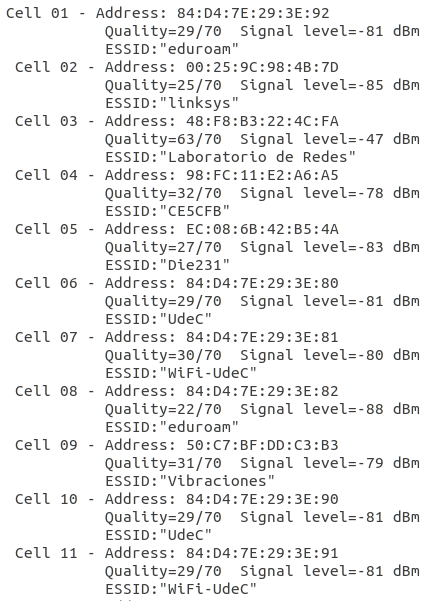
\includegraphics[width=.8\linewidth]{plaintext}  
  \caption{Salida de consola luego de medición}
  \label{fig:plaintext}
\end{subfigure}
\begin{subfigure}{.65\textwidth}
  \centering
  % include second image
  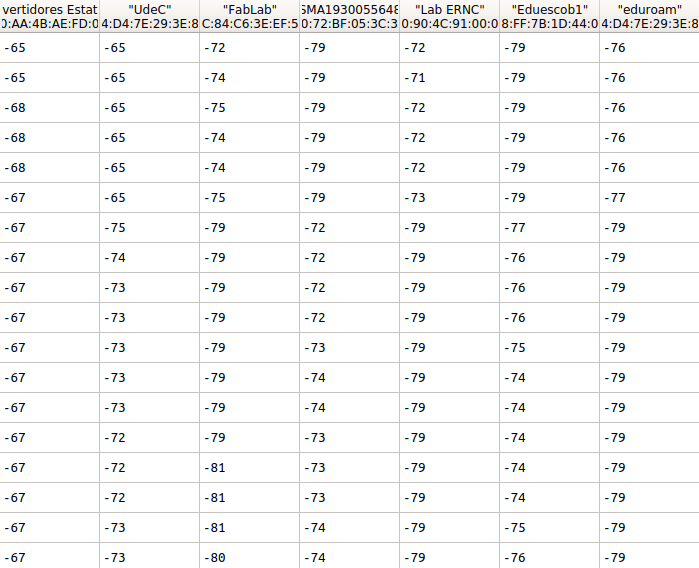
\includegraphics[width=.8\linewidth]{datossc}  
  \caption{Archivo depurado y transformado en .\texttt{csv}}
  \label{fig:plaincsv}
\end{subfigure}
\caption{Archivo antes y después de filtros sobre datos obtenidos}
\label{fig:tratdatos}
\end{figure}

A fin de estimar cuál era la cantidad idónea de muestras a tomar por ubicación, se optó por realizar un ensayo. Para esto, dividiendo el laboratorio en 4 sectores, se posicionó una raspberry en cada sector y se tomaron 5.000 muestras las cuales fueron trabajadas como se señaló en \ref{fig:tratdatos} añadiéndosele además una tupla que serían las coordenadas de posición en las que se habían tomado estas muestras. 

Luego, cuando se logró obtener un resultado que permitiera interpretar con qué precisión podía estimarse la posición usando 5.000 muestras para un número de 4 posiciones, se procedió a hacer lo mismo para un valor de muestra igual a 7.500, de este modo, se dedujo que para efectos de que la red capturara la mayor cantidad de características significantes de los datos, era necesario alimentarla con un mayor número de estos. 

% ###################################################################
% Para 9
% ###################################################################

Con la finalidad de precisar la información de posición del objetivo, se escaló en número, la cantidad de posiciones que se pueden estimar y considerando la conclusión a la que se había llegado luego del ensayo anterior, se aumentó la cantidad de datos, no sin antes, evaluar también el número óptimo de estos.

\begin{itemize}
    \item {10.000}
    \item {15.000}
    \item {20.000}
    \item {25.000}
    \item {30.000}
\end{itemize}


% Habiendo resuelto, como se mencionó, las salvedades, se procedió a estimar la posición del objetivo, en función de un vector de intensidad de señal medido.

\subsection{Laboratorio dividido en sectores.}

Tal y como se mencionó en \ref{fig:mapalab}, el laboratorio fue dividido en 9 sectores en los que se realizaron mediciones de potencia con una raspberry en cada ubicación.

Puntos a tratar en esta sección:
\begin{enumerate}
 \item {Cantidad apropiada de datos}
 \item{Tiempo que tarda la medición}
 \item{Tiempo que tarda el algoritmo de recolección de datos}
\end{enumerate}

\section{Entrenamiento}
\subsection{Ajustes entrenamiento}

\begin{enumerate}
    \item{Cantidad apropiada de neuronas}
    \item{Cantidad de epochs}
    \item{Tiempo que tarda el algoritmo de búsqueda de los mejores parámetros}
    \item{Tiempo que tarda el algoritmo que entrega la media del valor de precisión  de la red}
    \item{Tiempo que tarda la red en entrenarse con esos parámetros}
\end{enumerate}

\section{Predicción}

% \begin{itemize}
%     \item {\textbf{Etapa Offline}: }
%     \item {\textbf{Etapa Online}:}
% \end{itemize}